\documentclass[a4paper,t,xcolor=pst,dvips]{beamer}

\usepackage{beamerthemesplit}
\usepackage[utf8]{inputenc}
\usepackage[spanish]{babel}
\usepackage{graphicx}
\usepackage{pstricks} % PSTricks package
\usepackage{setspace}
\usepackage{multirow}
\usepackage{listings}
\usepackage{pgfpages}
\usepackage{hyperref}
\usepackage{etoolbox}
\usepackage{epstopdf}

\makeatletter
\patchcmd{\beamer@sectionintoc}{\vskip1.5em}{\vskip0.5em}{}{}
\makeatother

\setbeamercovered{dynamic}
\setcounter{tocdepth}{2}
\setbeamercolor{frametitle}{fg=black,bg=white}
\setbeamercolor{section in toc shaded}{fg=black}
\setbeamercolor{section in toc}{fg=red}
\setbeamercolor{subsection in toc shaded}{fg=black}
\setbeamercolor{subsection in toc}{fg=red}
\setbeamerfont{section in toc}{size=\small}
\setbeamerfont{subsection in toc}{size=\small}
\setbeamertemplate{section in toc shaded}[default][99]
\setbeamertemplate{subsection in toc shaded}[default][99]

\AtBeginSection[]
{\begin{frame}[c]
  \frametitle{Índice}
	\tableofcontents[currentsection,
        sectionstyle=show/shaded,
        subsectionstyle=hide]
\end{frame}}

\AtBeginSubsection[]
{\begin{frame}[c]
	\frametitle{Índice}
	\tableofcontents[
  		currentsection,
  		sectionstyle=shaded/shaded,
  		currentsubsection,
  		subsectionstyle=show/shaded/hide
		]
\end{frame}}

\setbeamercolor{frametitle}{fg=black,bg=white}

\setbeamertemplate{frametitle}{
	\begin{centering}
		\insertframetitle
		\par
	\end{centering}
}

\usetheme[secheader]{Boadilla} 

\newcommand{\imp}[1]{{\small{\sf #1}}}
\newcommand{\stk}{\emph{stakeholder}}

\title[Captura de Requisitos]{Procesos de Captura de Requisitos}

\author[P. Sánchez]{\alert{Pablo Sánchez}}

\institute[I2E]{
		   Dpto. Ingeniería Informática y Electrónica \\
		   Universidad de Cantabria \\
		   Santander (Cantabria, España) \\
		   p.sanchez@unican.es
}

\date{}

\begin{document}
	
\begin{frame}[c]
	\titlepage
	\begin{columns}
		\column{0.50\linewidth}
			\centering
    		
\includegraphics[width=.28\textwidth,keepaspectratio=true]{images/istr.eps}
		\column{0.50\linewidth}
			\centering
			
\includegraphics[width=.25\textwidth,keepaspectratio=true]{images/uc.eps}
	\end{columns}
\end{frame}

\begin{frame}[c]
    \frametitle{\alert{Advertencia}}
    \begin{center}
        Todo el material contenido en este documento  no constituye en modo alguno una obra de referencia o apuntes oficiales mediante el cual se puedan preparar las pruebas evaluables necesarias para superar la asignatura a la cual pertenecen. \ \\
        \ \\
        Este documento contiene exclusivamente una serie de diapositivas cuyo objetivo es servir de complemento visual a las actividades realizadas en el aula para la transmisión del contenido sobre el cual versarán las mencionadas pruebas evaluables.  \ \\
        \ \\
        Dicho de forma más clara, \alert{estas transparencias no son apuntes y su objetivo no es en modo alguno servir para que el alumno pueda preparar la asignatura.}
    \end{center}
\end{frame}

\section{Introducción}

\subsection{Objetivos}

\begin{frame}[c]
    \frametitle{Objetivos del Tema}
    \begin{enumerate}[<+->]
         \item Comprender cuáles son las diferentes etapas que conforman un \emph{proceso de captura de requisitos}.
         \item Saber utilizar técnicas frecuentemente utilizadas en las actividades de un proceso de captura de requisitos.
         \item Saber definir el \emph{contexto de un sistema software}.
         \item Saber identificar \emph{fuentes de requisitos} de un sistema sw.
         \item Saber seleccionar \emph{estrategias para la captura de requisitos}.
         \item Saber diseñar y ejecutar \emph la captura de requisitos.
    \end{enumerate}
\end{frame}

\subsection{Bibliografía}

\begin{frame}[c]
    \frametitle{Bibliografía}
    \begin{thebibliography}{1}

    \bibitem{pohl:2010a} Klaus Pohl. \newblock {\em {Requirements Engineering: Fundamentals, Principles and Techniques}}.
    \newblock Springer, June 2010.

    \bibitem{cockburn:2000} Alistair Cockburn. \newblock {\em {Writing Effective Use Cases}}.
    \newblock Addison-Wesley, October 2000.

    \bibitem{gray:2012}
    Gray, D., Brown, S., and Macanufo, J. (2012).
    \newblock {\em {Gamestorming: 83 juegos para innovadores, inconformistas y generadores del cambio}}.
    \newblock Deusto.
\end{thebibliography}
\end{frame}

\subsection{Procesos de Captura de Requisitos}

\begin{frame}
    \frametitle{Proceso de Ingeniería de Requisitos}
    \only<1>{
	\rput[lt](0,-0.5){
	   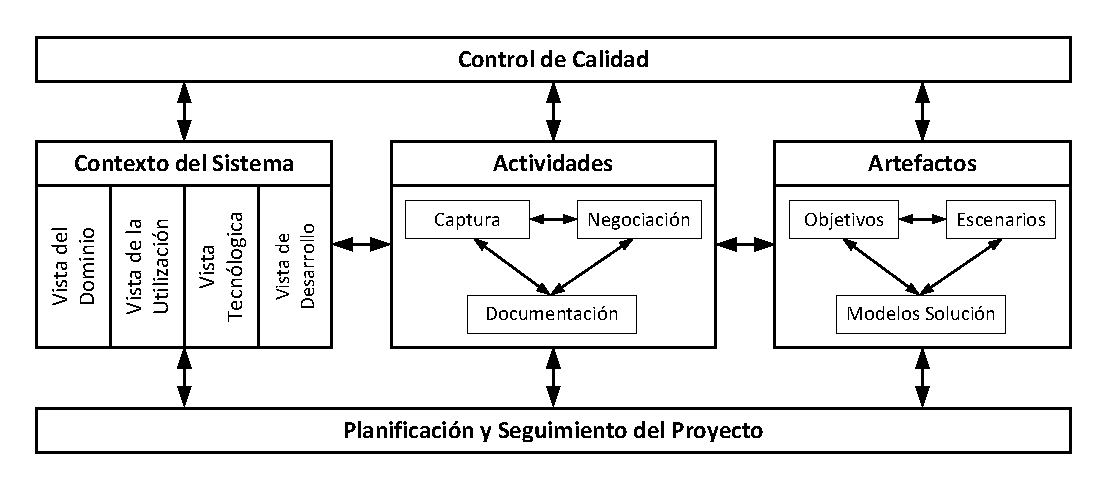
\includegraphics[width=11.5cm,keepaspectratio=true]{images/introduction/procesoIr00.eps}}
	}
    \only<2>{
	\rput[lt](0,-0.5){
	   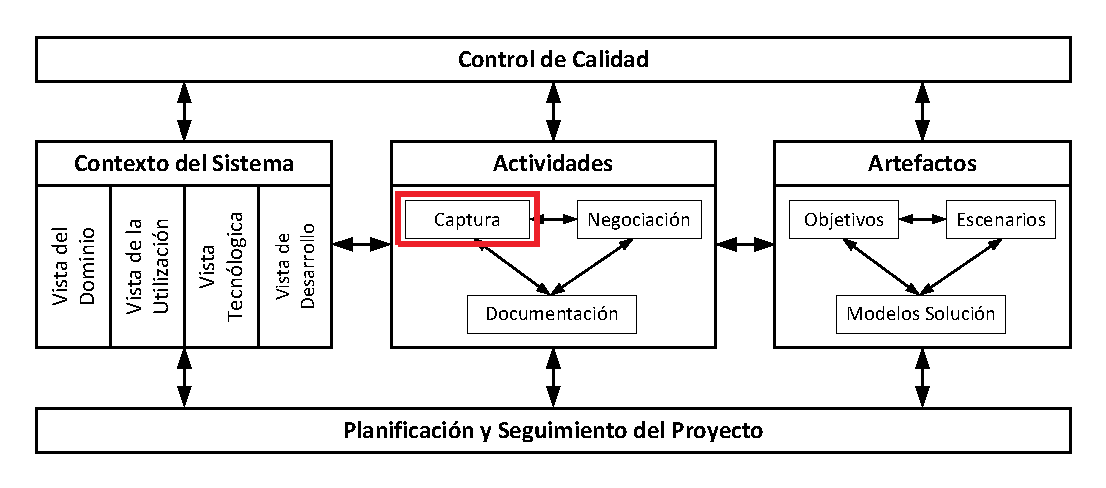
\includegraphics[width=11.5cm,keepaspectratio=true]{images/introduction/procesoIr01.eps}}
	}
\end{frame}

\begin{frame}
    \frametitle{Proceso de Captura de Requisitos}
    \begin{center}
        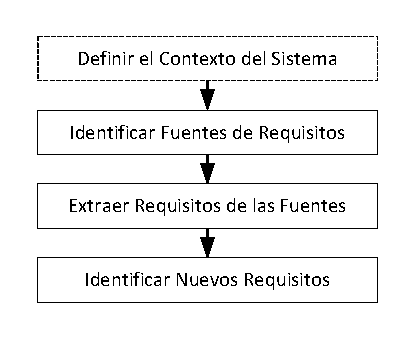
\includegraphics[width=0.75\linewidth]{images/introduction/procesoCaptura.eps}
    \end{center}
\end{frame}

\section{Técnicas Base}

\subsection{Tormenta de Ideas}

\begin{frame}[t]
    \frametitle{Tormenta de Ideas - Fundamento}
    \begin{block}{Tormenta de Ideas}
        \begin{enumerate}[<+->]
            \item Varias personas se reúnen en una sala para expresar públicamente sus ideas sobre un asunto concreto.
            \item Las ideas no necesitan estar elaboradas, ni ser aplicables en la realidad.
            \item Un participante puede utilizar las ideas propuestas por otros para construir nuevas ideas.
        \end{enumerate}
    \end{block}
\end{frame}

\begin{frame}[c]
    \frametitle{Tormenta de Ideas - Preparación}
    \begin{enumerate}[<+->]
        \item Definir con claridad el \alert{objetivo} de la sesión.
        \item Seleccionar con exhaustividad los integrantes adecuados para alcanzar el objetivo.
        \item Reservar una sala adecuada y fijar la hora de la sesión.
        %% Sala adecuada: Todos se ven las caras y debe disponer de un medio para visualizar los resultados
        \item Notificar lugar y hora a los participantes.
        \item Preparar el mecanismo de visualización.
        \item Seleccionar un moderador y un secretario.
    \end{enumerate}
\end{frame}

\begin{frame}[c]
    \frametitle{Tormenta de Ideas - Ejecución}
    \begin{enumerate}[<+->]
        \item Prima la cantidad sobre la calidad.
        \item Asociación libre de ideas e imaginación.
        \item Combinar ideas.
        \item Las críticas (destructivas) no están permitidas.
        \item Se pueden pedir aclaraciones sobre las ideas expuestas.
        \item No interrumpir la sesión al primer silencio largo.
        \item Dejar que la sesión termine de forma natural, sin controlar el tiempo.
    \end{enumerate}
\end{frame}

\begin{frame}[c]
    \frametitle{Tormenta de Ideas - Resultados}
    \begin{enumerate}[<+->]
        \item Clasificar las ideas (utilizables, probablemente útiles, no útiles).
        \item Descartar las ideas no utilizables.
        \item Elaborar un plan para desarrollar las ideas utilizables.
        \item Elaborar un documento que resuma la sesión y recoja los resultados.
    \end{enumerate}
\end{frame}

\subsection{Método KJ}

\begin{frame}[t]
	\frametitle{Método KJ - Fundamento}
	\begin{block}{Método KJ}
		\begin{enumerate}
			\item Cada participante describe sus ideas sobre un asunto concreto en una o más tarjetas de papel, destacando las palabras claves.
			\item Las ideas se agrupan por categoría.
			\item Los participantes seleccionan las mejores ideas, las cuales se refinan más tarde.
		\end{enumerate}
	\end{block}
\end{frame}

\begin{frame}[c]
	\frametitle{Método KJ - Preparación}
	\begin{enumerate}[<+->]
		\item Definir con claridad el \alert{objetivo} de la sesión.
		\item Seleccionar con exhaustividad los integrantes adecuados para alcanzar el objetivo.
		\item Reservar una sala adecuada y fijar la hora de la sesión.
		%% Sala adecuada: Todos se ven las caras y debe disponer de un medio para visualizar los resultados
		\item Notificar lugar y hora a los participantes.
		\item Preparar el mecanismo de visualización.
		\item Seleccionar un moderador y un secretario.
	\end{enumerate}
\end{frame}

%% Revisar
\begin{frame}[c]
	\frametitle{Método KJ - Ejecución (I)}
	\begin{enumerate}[<+->]
		\item Explicar con claridad el objetivo de la sesión.
		\item Explicar las reglas del juego y mostrar una tarjeta de ejemplo.
		\item Repartir las tarjetas y bolígrafos.
		\item Establecer un tiempo para la elaboración de las ideas.
		\item Colocar las tarjetas sobre un tablero, numerándolas.
		\item Permitir a los participantes explicar sus tarjetas si eso fuese necesario.
	\end{enumerate}
\end{frame}

\begin{frame}[c]
	\frametitle{Método KJ - Ejecución (II) y Resultados}
	\begin{enumerate}[<+->]
		\item Agrupar las tarjetas por categorías, sin eliminar las tarjetas.
		\item Establecer de manera cooperativa un título para cada categoría.
		\item Establecer, si fuese necesario, relaciones entre categorías.
		\item Determinar un plan de acción.
		\item Documentar la sesión y distribuir los resultados.
	\end{enumerate}
\end{frame}

\subsection{Prototipado}

\begin{frame}[t]
    \frametitle{Prototipado - Fundamento}
    \begin{block}{Prototipado}
        Se construyen prototipos con los que diversos \emph{stakeholders} puedan interactuar para analizar su reacción, así como para comprobar que dichos prototipos satisfacen sus necesidades.
    \end{block}
\end{frame}

\begin{frame}[c]
    \frametitle{Prototipos - Preparación}
    %% Los prototipos escenifican las consecuencias de los requisitos a los stakeholders
    %% Prototipos desechables y evoluvitos
    %% Mock-up
    \begin{enumerate}[<+->]
        \item Decidir el momento de la creación del prototipo.
        \item Definir escenarios de utilización del prototipo, y decidir qué requisitos debe satisfacer el prototipo.
        \item Elegir el tipo de prototipo a construir: evolutivo o desechable.
        \item En función del tipo de prototipo, elegir la técnica más adecuada de elaboración.
        \item Seleccionar una herramienta adecuada para la elaboración del prototipo.
    \end{enumerate}
\end{frame}

\begin{frame}[c]
    \frametitle{Prototipos - Ejecución y Resultados}
    \begin{enumerate}[<+->]
        \item Hacer que los \emph{stakeholders} interactúen con el prototipo un tiempo suficiente.
        \item Recopilar datos acerca de cómo los \emph{stakeholders} interactúan con los prototipos, así como de sus reacciones.
        %% Eye-tracking
        \item Analizar los datos recogidos.
    \end{enumerate}
\end{frame}


\subsection{Mapas Mentales}

\begin{frame}[t]
    \frametitle{Mapas mentales - Fundamento}
    \begin{block}{Mapa mental}
        \begin{enumerate}[<+->]
            \item Técnica de representación gráfica del conocimiento relacionado con un \alert{tema concreto}.
            \item Cada tema se descompone en una serie de subtemas o palabras claves.
            \item Cada subtema o palabra clave se puede descomponer en una serie de subtemas o palabras claves, y así sucesivamente.
            \item Los subtemas de un tema o palabra clave se pueden relacionar con temas o palabras claves de otros temas o subtemas.
            \item Los diversos conocimientos relacionados con un tema aparecen como nodos de una red de nodos interrelacionados.
            \item Se estimula la capacidad verbal del lado izquierdo del cerebro y la capacidad visual y espacial del lado derecho.
        \end{enumerate}
    \end{block}
\end{frame}

\begin{frame}[c]
    \frametitle{Mapas mentales - Fundamento}
    \begin{center}
        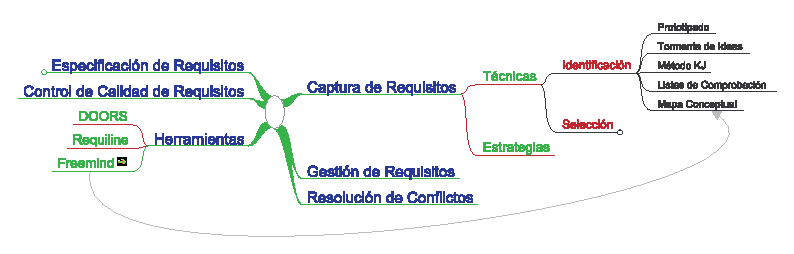
\includegraphics[width=\linewidth]{images/tecnicas/mapaConceptual.eps}
    \end{center}
\end{frame}

\begin{frame}[c]
    \frametitle{Mapas mentales - Preparación y Ejecución}
    \begin{block}{Preparación}
    \begin{enumerate}[<+->]
        \item Elegir el medio (herramienta sw, papel, pizarra (electrónica)) para la realización del mapa mental.
    \end{enumerate}
    \end{block}
    \uncover<2->{
    \begin{block}{Ejecución}
    \begin{enumerate}[<+->]
        \item Mapas mentales
        \item Subdividir el tema central en subtemas o palabras claves.
        \item Refinar cada una de las palabras claves hasta alcanzar el objetivo deseado.
        \item Relacionar las palabras claves de diferentes subtemas si fuese necesario.
        \item Adornar el mapa con iconos y colores.
    \end{enumerate}
    \end{block}
    }
\end{frame}

\begin{frame}[t]
    \frametitle{Mapas mentales - Resultados}
    \begin{block}{Resultados}
    \begin{enumerate}[<+->]
        \item Reorganizar la disposición espacial si fuese necesario.
        \item Incluir las aclaraciones que se consideren pertinentes.
    \end{enumerate}
    \end{block}
\end{frame}

\subsection{Listas de Control}

\begin{frame}[t]
    \frametitle{Listas de Control - Fundamento}
    \begin{block}{Listas de Control}
        \begin{enumerate}[<+->]
            \item Una \emph{lista de control} contiene varios puntos, redactados en forma de preguntas o sentencias, acerca de un cierto tema.
            \item Sirven para comprobar una serie de elementos relacionados con un tema recurrente.
            \item Favorecen que no se obvie o olvide ninguno de estos puntos.
        \end{enumerate}
    \end{block}
\end{frame}

\begin{frame}[c]
    \frametitle{Listas de control - Preparación, Ejecución y Resultados}
    \begin{block}{Preparación}
    \begin{enumerate}[<+->]
        \item Elegir un lista de control de entre el catálogo de listas existentes.
        \item Si no existiese una determinada lista de control, crearla utilizando el procedimiento adecuado para ello (e.g., tormenta de ideas).
    \end{enumerate}
    \end{block}
    \uncover<3->{
    \begin{block}{Ejecución}
    \begin{enumerate}[<+->]
        \item Revisar y procesar cada uno de los puntos de control.
        \item Si se detectasen inconsistencias, imprecisiones, ambigüedades, redundancias o carencias, notificarlo.
    \end{enumerate}
    \end{block}
    }
    \uncover<5->{
    \begin{block}{Resultados}
    \begin{enumerate}[<+->]
        \item Actualizar la lista de control si fuese necesario.
    \end{enumerate}
    \end{block}
    }
\end{frame}

\subsection{Test 100\$}


\begin{frame}[t]
    \frametitle{100\$ Test - Fundamento}
    \begin{block}{100\$ Test}
        \begin{enumerate}
            \item<1-> Sistema colaborativo para la elección de elementos de una lista, o para ordenar una lista de elementos por prioridad o relevancia.
            \item<2-> Se asigna \emph{dinero virtual} a cada miembro del grupo.
            \item<3-> Cada miembro invierte dinero en función de su criterio personal.
            \item<4-> La inversión colectiva se considera la más adecuada, y por tanto la elegida.
        \end{enumerate}
    \end{block}
\end{frame}

\begin{frame}[c]
    \frametitle{100\$ Test - Preparación}
    \begin{enumerate}[<+->]
        \item Definir la lista de elementos a ordenar o filtrar.
        \item Decidir si se usará un sistema con acumulación o sin acumulación.
    \end{enumerate}
\end{frame}

\begin{frame}[c]
    \frametitle{100\$ Test - Ejecución}
    \begin{enumerate}[<+->]
        \item Asignar dinero virtual a cada miembro del grupo. Un tercio de la longitud de la lista de elementos a procesar en sistemas sin acumulación, la mitad en sistemas con acumulación.
        \item Cada participante reparte su dinero entre los elementos de la lista.
        \item En sistemas sin acumulación, sólo se puede asignar un dólar a cada elemento.
        \item En sistemas con acumulación, se puede asignar más un dólar a un elemento, hasta un máximo establecido.
        \item Se recogen las apuestas y se procesan.
    \end{enumerate}
\end{frame}

\begin{frame}[c]
    \frametitle{100\$ Test - Resultados}
    \begin{enumerate}[<+->]
        \item Ordenar los elementos en función de la cantidad de dinero recibida.
        \item Si se pretende filtrar o seleccionar un conjunto de elementos, establecer un criterio de corte claramente definido.
        \item En caso de querer ordenarlos por relevancia, se puede aplicar alguna técnica para deshacer los empates; o se pueden agrupar los elementos por niveles, donde todos los elementos de un nivel son de igual prioridad.
    \end{enumerate}
 \end{frame}



\section{Definición del Contexto de un Sistema Sw}

\subsection{Contexto y Frontera de un Sistema Sw}

\begin{frame}[c]
    \frametitle{Contexto de un Sistema Sw}
    \begin{center}
        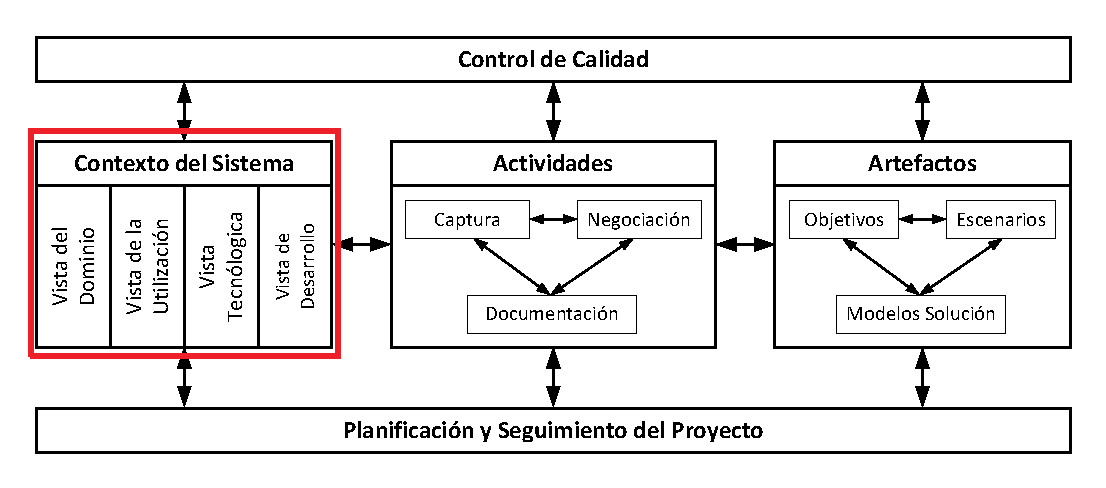
\includegraphics[width=\linewidth]{images/contexto/procesoIrContexto.eps}
    \end{center}
\end{frame}

\begin{frame}[c]
    \frametitle{Contexto de un Sistema Sw}
    \begin{center}
        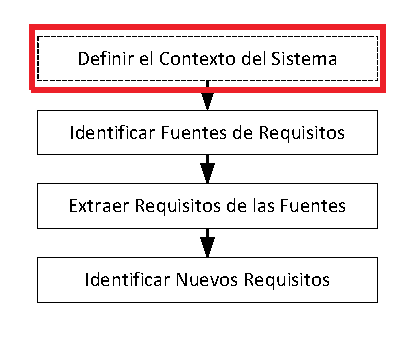
\includegraphics[width=0.65\linewidth]{images/contexto/procesoCapturaContexto.eps}
    \end{center}
\end{frame}

\begin{frame}[c]
    \frametitle{Contexto y Frontera de un Sistemas Sw}
    \begin{block}{Contexto de un Sistema Sw~\cite{pohl:2010}}
        El \alert{\emph{contexto de un sistema sw}} es la parte del entorno de dicho sistema sw que es de relevancia para la definición, comprensión e interpretación de los requisitos de un sistema.
    \end{block}
    \uncover<2->{
    \begin{block}{Frontera de un Sistema Sw~\cite{pohl:2010}}
        La \alert{\emph{frontera de un sistema sw}} separa el sistema sw bajo desarrollo (o desarrollado) del contexto del sistema.
        %% Aclarar aquí que el sistema puede ser modificado, mientras que el contexto no puede serlo
    \end{block}
    }
    \uncover<3->{
    \begin{block}{Frontera de un Contexto Sw~\cite{pohl:2010}}
        La \alert{\emph{frontera de un contexto sw}} separa la parte relevante del contexto de un sistema de la parte irrelevante.
        %% Leyes y normas
    \end{block}
    }
\end{frame}

\begin{frame}[c]
    \frametitle{Contexto y Frontera de un Sistema Sw}
    \begin{center}
        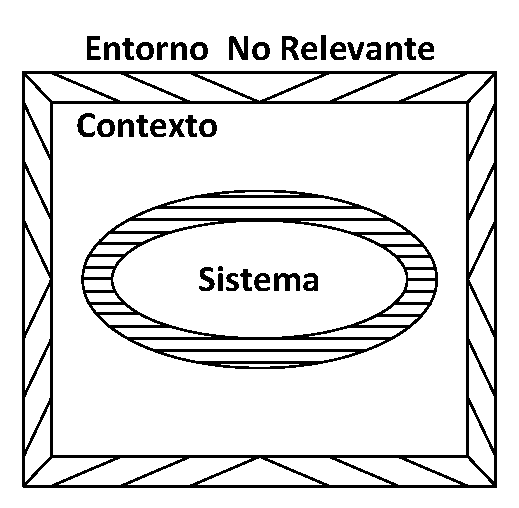
\includegraphics[width=0.50\linewidth]{images/contexto/contexto.eps}
    \end{center}
\end{frame}

\subsection{Estructura del Contexto de un Sistema Sw}

\begin{frame}[c]
    \frametitle{Estructura del Contexto de un Sistema Sw}
    \begin{center}
        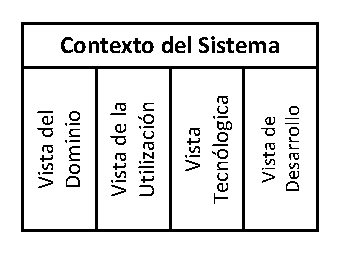
\includegraphics[width=0.30\linewidth]{images/contexto/estructuraContexto.eps}
    \end{center}
    \uncover<2->{
    \begin{description}
        \item<2->[Vista del Dominio] Objetos y eventos que son relevantes para el sistema sw.
        \item<3->[Vista de la Utilización] Cómo los usuarios (personas o sistemas) utilizan el sistema sw para satisfacer un objetivo.
        \item<4->[Vista Tecnológica] La infraestructura tecnológica donde se despliega el sistema sw.
        \item<5->[Vista de Desarrollo] Cómo debe desarrollarse el sistema sw.
    \end{description}
    }
\end{frame}

\subsection{Definición del Contexto de un Sistema Sw}

\begin{frame}[c]
    \frametitle{Definición del Contexto de un Sistema Sw}
    \begin{enumerate}[<+->]
        \item Definir la \emph{visión del sistema}.
        \item Crear un glosario con los elementos importantes del contexto del sistema.
        \item Definir la \emph{frontera del sistema} y la \emph{frontera del contexto}.
    \end{enumerate}
\end{frame}

\begin{frame}[c]
    \frametitle{Definición de la Frontera del Sistema}
    \begin{enumerate}[<+->]
        \item Involucrar en el proceso a todos los \emph{stakeholders}.
        \item Decidir qué elementos pertenecen al sistema.
        \item Decidir qué elementos no pertenecen al sistema.
        \item En caso de dudas, asignar el elemento a la \emph{zona gris}.
        \item Revisar periódicamente la frontera del sistema. Si algún elemento cambia de zona, revisar los requisitos afectados.
    \end{enumerate}
\end{frame}

\begin{frame}[c]
    \frametitle{Definición de la Frontera del Contexto}
    \begin{enumerate}[<+->]
        \item Involucrar en el proceso a todos los \emph{stakeholders}.
        \item Decidir qué elementos pertenecen a cada una de las cuatro vistas del contexto.
        \item En caso de dudas, asignar el elemento a la \emph{zona gris}.
        \item Revisar periódicamente la frontera del contexto. Si algún elemento cambia de zona, revisar los requisitos afectados.
    \end{enumerate}
\end{frame}

\begin{frame}[c]
     \frametitle{Listas Dentro/Fuera}
     \begin{center}
     \begin{tabular}{||l||c|c|c||}
     \hline \hline
     \textbf{Elemento}          & \textbf{Sistema} & \textbf{Contexto} & \textbf{Irrelevante} \\ \hline \hline
     Notificar Fin Reparación   &   $\checkmark$   &                   &                      \\ \hline
     Generar Factura            &   $\checkmark$   &                   &                      \\ \hline
     Generar Trimestral IVA     &   $\checkmark$   & $\checkmark$      &                      \\ \hline
     Comunicación Proveedores   &                  & $\checkmark$      &                      \\ \hline
     Plan RENOVE                &                  &                   & $\checkmark$         \\ \hline
     \hline
     \end{tabular}
     \end{center}
\end{frame}

\section{Fuentes para la Captura de Requisitos}

\begin{frame}[c]
	\frametitle{Fuentes para la Captura de Requisitos}
	\begin{center}
		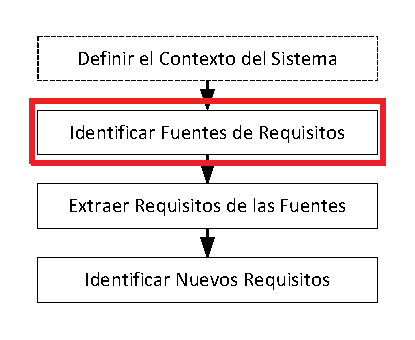
\includegraphics[width=0.75\linewidth]{images/proceso/fuentes.eps}
	\end{center}
\end{frame}

\subsection{Tipos de Fuentes de Requisitos}

\begin{frame}[c]
	\frametitle{Fuentes Habituales de Requisitos}
	\begin{itemize}[<+->]
		\item Stakeholders.
		\begin{itemize}[<+->]
			\item Usuarios (los que lo usan).
			\item Clientes (los que costean su desarrollo).
			\item Analistas de mercados.
			\item Entidades reguladoras.
			\item Ingenieros Sw.
		\end{itemize}
		\item Documentos.
		\item Sistemas e infraestructura actualmente existentes.
	\end{itemize}
\end{frame}

\subsection{Proceso de Identificación de Fuentes de Requisitos}

\begin{frame}[c]
	\frametitle{Proceso de Identificación de Fuentes}
	\begin{enumerate}
		\item<1-> Seleccionar las fuentes obvias (e.g., documento con la visión del sistema) (listas de comprobación).
		\item<2-> Identificar nuevas fuentes mediante el análisis de:
		\begin{enumerate}
			\item<3-> \emph{Stakeholders} identificados.
			\item<4-> Documentos identificados.
			\item<5-> Análisis de sistemas actualmente existentes.
		\end{enumerate}
		\item<6-> Registrar las nuevas fuentes identificadas. Si el número de nuevas fuentes detectadas es suficientemente bajo, ir al paso 5.
		\item<7-> Por cada nueva fuente identificada, repetir el paso 2.
		\item<8-> Seleccionar aquellas fuentes que se consideren de mayor relevancia.
	\end{enumerate}
\end{frame}

\section{Estrategias para la Identificación de Requisitos}

\begin{frame}[c]
	\frametitle{Identificación de Requisitos Existentes}
	\begin{center}
		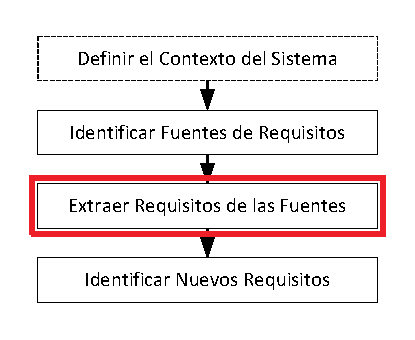
\includegraphics[width=0.75\linewidth]{images/proceso/requisitosViejos.eps}
	\end{center}
\end{frame}

\begin{frame}[c]
	\frametitle{Identificación de Nuevos Requisitos}
	\begin{center}
		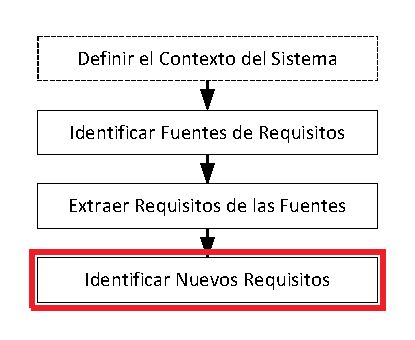
\includegraphics[width=0.75\linewidth]{images/proceso/requisitosNuevos.eps}
	\end{center}
\end{frame}

\subsection{Entrevistas}

\begin{frame}[t]
    \frametitle{Entrevistas - Fundamento}
    \begin{block}{Tipos de Entrevistas}
        \begin{description}[<+->]
            \item[Estandarizada] Existen unas preguntas predefinidas de las que el entrevistador no se puede desvíar.
            \item[Exploratoria] Existen unas preguntas predefinidas de las que el entrevistador se puede desvíar.
            \item[No estructurada] No existen preguntas predefinidas.
        \end{description}
    \end{block}
\end{frame}

\begin{frame}[c]
    \frametitle{Entrevistas - Preparación del Evento}
    \begin{enumerate}[<+->]
        \item Definir claramente el objetivo de la reunión.
        \item Elegir los participantes para la entrevista.
        \item Elegir un sitio adecuado (aislado y sin ruidos) para realizar las entrevistas.
        \item Invitar a los participantes con antelación suficiente.
        \item Explicar el objetivo y procedimiento a los participantes.
    \end{enumerate}
\end{frame}

\begin{frame}[t]
    \frametitle{Entrevistas - Preparación de la Entrevista}
    \begin{block}{Preparación de la Entrevista}
    \begin{enumerate}[<+->]
        \item Utilizar preguntas cerradas y abiertas según convenga.
        \item Precisar un contexto para cada pregunta si ello fuese necesario.
        \item Evitar preguntas \emph{sugerentes}.
    \end{enumerate}
    \end{block}
    \uncover<4->{
    \begin{block}{Preparación del Entrevistador}
    \begin{enumerate}
        \item<4-> Familiarizarse con los entrevistados.
        \item<5-> Familiarizarse con la terminología propia de los entrevistados y utilizarla.
    \end{enumerate}
    \end{block}
    }
\end{frame}

\begin{frame}[c]
    \frametitle{Entrevistas - Ejecución}
    \begin{enumerate}[<+->]
        \item Al principio, repasar el objetivo y proporcionar información adicional (si fuese necesario).
        \item Realizar una pregunta introductoria.
        \item Ligar las respuestas recibidas con las preguntas para corroborar que la información recibida es correcta.
        \item Crear modelos y escenarios para verificar que la información recibida es correcta.
        \item Examinar la \emph{comunicación no verbal} de los entrevistados.
        \item Realizar descansos cortos (5-10m.) tras 45m de entrevista.
        \item No irse por las ramas ni perderse en detalles.
        \item Agradecer a los entrevistados su participación al final y comentar su importancia.
    \end{enumerate}
\end{frame}

\begin{frame}[c]
    \frametitle{Entrevistas - Resultados}
    \begin{enumerate}[<+->]
        \item Documentar y archivar  de los resultados.
        \item Revisar los modelos creados.
        \item Recopilar las cuestiones a aclarar y tareas pendientes.
        \item Enviar los resultados a los entrevistados.
        \item Solicitar a los entrevistados que confirmen los resultados.
        \item Analizar conflictos y resolverlos.
    \end{enumerate}
\end{frame}

\subsection{Cuestionarios}

\begin{frame}[c]
	\frametitle{Cuestionarios - Preparación y Ejecución}
	\begin{block}{Preparación}
		\begin{enumerate}
			\item<1-> Definir claramente el objetivo del cuestionario.
			\item<2-> Definir los resultados esperados.
			\item<3-> Seleccionar a los \emph{stakeholders} que completarán el cuestionario.
			\item<4-> Elaborar las preguntas del cuestionario.
		\end{enumerate}
	\end{block}
	\uncover<5->{
		\begin{block}{Ejecución}
			\begin{enumerate}
				\item<5-> Aclarar a los \emph{stakeholders} el objetivo final del cuestionario.
				\item<6-> Establecer una fecha límite para completar el cuestionario.
				\item<7-> Proporcionar un mecanismo de contacto para la resolución de dudas durante el cumplimiento del formulario.
				\item<8-> Agradecer a los participantes su colaboración.
			\end{enumerate}
		\end{block}
	}
\end{frame}

\begin{frame}[t]
	\frametitle{Cuestionarios - Resultados}
	\begin{block}{Resultados}
		\begin{enumerate}[<+->]
			\item Procesar las respuestas.
			\item Clarificar las respuestas ambiguas, siempre que sea posible.
			\item Prestar especial atención a los conflictos entre requisitos.
			\item Comunicar los resultados a los participantes.
		\end{enumerate}
	\end{block}
\end{frame}

\subsection{Grupos de Interés}

\begin{frame}[t]
    \frametitle{Grupos de Interés - Fundamento}
    \begin{block}{Grupo de Interés para la Captura de Requisitos}
        Se reúne un grupo de \emph{stakeholders}, expertos en una determinada área, los cuales debaten para dar respuesta a una pregunta planteada.
    \end{block}

    %%============================================================================================%%
    %% NOTA(Pablo):  Esto considero que no es relevante
    %%============================================================================================%%
    %%
    %%    \uncover<2->{
    %%    \begin{block}{Tipos de Grupos de Interés}
    %%        \begin{description}
    %%            \item<2->[Exploratorio] Orientado a identificar nuevos requisitos.
    %%            \item<3->[Comparativo] Se compara el sistema bajo desarrollo con otro existente.
    %%            \item<4->[Priorización] Se ordenan requisitos ya capturados por prioridad
    %%        \end{description}
    %%    \end{block}
    %%    }
    %%============================================================================================%%

\end{frame}

\begin{frame}[c]
    \frametitle{Grupos de Interés - Preparación}
    \begin{enumerate}[<+->]
        \item Definir claramente el objetivo y el elemento de interés.
        \item Seleccionar los participantes adecuados.
        \item Reservar una sala adecuada (sin ruidos y con equipamiento).
        \item Elegir a un moderador y secretario (externos).
        \item Invitar a los participantes con antelación, explicando el objetivo (negociable).
    \end{enumerate}
\end{frame}

\begin{frame}[t]
    \frametitle{Grupos de Interés - Ejecución}
    \begin{enumerate}[<+->]
        \item Recibir a los participantes.
        \item Abrir con una pregunta inicial.
        \item Fomentar la participación de todos los miembros.
        \item Evitar discusiones acaloradas y periodos largos de silencio.
        \item El secretario levanta acta, documentando las decisiones adoptadas.
        \item Agradecer a los participantes su asistencia y participación.
    \end{enumerate}
\end{frame}

\begin{frame}[t]
    \frametitle{Grupos de Interés - Resultados}
    \begin{enumerate}[<+->]
        \item Elaborar el acta e informe de resultados definitivo.
        \item Enviar dichos documentos a los participantes para su aprobación.
        \item Recopilar y procesar las cuestiones que hayan quedado abiertas.
    \end{enumerate}
\end{frame}

\subsection{Talleres}

\begin{frame}[t]
	\frametitle{Talleres - Fundamento}
	\begin{block}{Taller de Captura de Requisitos}
		Se reúne un grupo de \emph{stakeholders}, los cuales trabajan conjuntamente, durante una o más jornadas y mediante diversas actividades de grupo, para dar respuesta a una serie de preguntas planteadas. Dichas respuestas permiten obtener una serie de requisitos que ha de satisfacer el sistema bajo desarrollo.
	\end{block}
\end{frame}

\begin{frame}[c]
	\frametitle{Talleres - Preparación}
	\begin{enumerate}[<+->]
		\item Definir claramente el objetivo del taller.
		\item Definir los resultados esperados.
		\item Diseñar un método de trabajo adecuado para alcanzar los objetivos.
		\item Elaborar la \alert{\emph{agenda}} del taller (incluir descansos).
		\item Seleccionar los participantes de forma que haya hetereogeneidad y teniendo en cuenta el objetivo.
		\item Invitar a los participantes con antelación, explicando el objetivo (negociable).
		\item Reservar una sala adecuada (sin ruidos y con equipamiento).
		\item Elegir a un moderador y secretario (externos).
	\end{enumerate}
\end{frame}

\begin{frame}[t]
	\frametitle{Talleres - Ejecución}
	\begin{enumerate}[<+->]
		\item Presentar y debatir el objetivo, los resultados esperados y la agenda.
		\item Explicar las actividades (de grupo) a realizar.
		\item Explicar y votar las reglas que regirán el desarrollo del taller.
		\item El moderador controla las actividades y el cumplimiento de las reglas.
		\item El secretario levanta acta de los resultados intermedios y finales obtenidos, documentando las decisiones adoptadas.
		\item Se debe prestar especial atención a los conflictos.
		\item Recopilar todas las cuestiones que hayan quedado abiertas.
		\item Definir un procedimiento a seguir para cada cuestión.
		\item Recoger datos sobre la productividad del taller para su mejora.
		\item Agradecer a los participantes su asistencia y participación.
	\end{enumerate}
\end{frame}

\begin{frame}[t]
	\frametitle{Talleres - Resultados}
	\begin{enumerate}[<+->]
		\item Elaborar el acta e informe de resultados definitivo.
		\item Enviar dichos documentos a los participantes para su aprobación.
	\end{enumerate}
\end{frame}

\subsection{Observación}

\begin{frame}[t]
    \frametitle{Observación - Fundamento}
    \begin{block}{Tipos de Observación}
        \begin{description}
            \item[Directa] El observador observa y analiza como se comportan los \emph{stakeholders}.
            \item[Etnográfica] El observador aprende a realizar y realiza las tareas propias de un \emph{stakeholder}.
        \end{description}
    \end{block}
\end{frame}

\begin{frame}[c]
    \frametitle{Observación - Preparación y Ejecución}
    \begin{block}{Preparación de una Observación}
        \begin{enumerate}
            \item<1-> Definir claramente el objetivo de la observación.
            \item<2-> Definir los elementos que deben ser observados.
            \item<3-> Definir los resultados esperados.
        \end{enumerate}
    \end{block}
    \uncover<4->{
        \begin{block}{Ejecución de una Observación}
            \begin{enumerate}
                \item<4-> Ganarse la confianza de los \emph{stakeholders}.
                \item<5-> Observar con detalle el comportamiento de los \emph{stakeholders}.
                \item<6-> Documentar los elementos de interés tal como sucedan (texto, audio o vídeo).
                \item<7-> Verificar la objetividad y autenticidad de los resultados.
            \end{enumerate}
        \end{block}
    }
\end{frame}

\begin{frame}[t]
    \frametitle{Observación - Resultados}
    \begin{enumerate}[<+->]
        \item Elaborar un informe final de resultados conforme los estándares establecidos.
        \item Vincular los resultados con los \emph{stakeholders} que los produjeron.
        \item Vincular los requisitos capturados con la correspondiente fuente.
    \end{enumerate}
\end{frame}


\subsection{Lectura en Perspectiva}

\begin{frame}[c]
    \frametitle{Lectura con perspectiva - Preparación y Ejecución}
    \begin{block}{Lectura con perspectiva - Fundamento}
        Un determinado lector analiza un documento concreto desde una determinada perspectiva, analizando los detalles que son relevantes desde esa perspectiva e ignorando los irrelevantes.
    \end{block}
    \uncover<2->{
        \begin{block}{Preparación}
            \begin{enumerate}
                \item<2-> Definir claramente el objetivo de las lecturas.
                \item<3-> Definir las perspectivas.
                \item<4-> Seleccionar los documentos a analizar.
                \item<5-> Seleccionar a los lectores y avisarlos con antelación.
            \end{enumerate}
        \end{block}
    }
\end{frame}

\begin{frame}[t]
    \frametitle{Lectura con perspectiva - Resultados}
    \begin{block}{Ejecución}
        \begin{enumerate}
            \item<1-> Seleccionar una técnica para analizar los documentos (secuencial o dirigida).
            \item<2-> Vincular los requisitos identificados con los pasajes de texto correspondientes.
        \end{enumerate}
    \end{block}
    \uncover<3->{
        \begin{block}{Resultados}
            \begin{enumerate}
                \item<3-> Elaborar un informe de resultados.
                \item<4-> Prestar especial atención a los conflictos entre requisitos.
            \end{enumerate}
        \end{block}
    }
\end{frame}

\subsection{Resumen}

\begin{frame}[c]
	\frametitle{Resumen Técnicas Básicas}
	\begin{center}
		\begin{tabular}{||l|l|c|c|c||}
			\hline \hline
			\textbf{Técnica}  & \textbf{Coste} & \textbf{Fuentes} & \textbf{Existentes} & \textbf{Nuevos} \\ \hline \hline
			Tormenta de Ideas & Bajo           & $\checkmark$     &                     & $\checkmark$    \\ \hline
			Prototipado       & Variable       &                  & $\checkmark$        & $\checkmark$    \\ \hline
			Método KJ         & Bajo           & $\checkmark$     & $\checkmark$        & ($\checkmark$)  \\ \hline
			Mapa Mental       & Bajo           & $\checkmark$     & $\checkmark$        & $\checkmark$  \\ \hline
			Listas de Control & Bajo           & $\checkmark$     & $\checkmark$        & $\checkmark$  \\ \hline \hline
		\end{tabular}
	\end{center}
\end{frame}

\begin{frame}[c]
    \frametitle{Resumen Técnicas de Identificación}
    \begin{center}
    \begin{tabular}{||l|l|c|c|c||}
        \hline \hline
        \textbf{Técnica}    & \textbf{Coste} & \textbf{Fuentes} & \textbf{Existentes} & \textbf{Nuevos} \\ \hline \hline
        Entrevistas         & Medio-Alto     & $\checkmark$     & $\checkmark$        & $\checkmark$    \\ \hline
        Talleres            & Alto-Muy Alto  & $\checkmark$     & $\checkmark$        & $\checkmark$    \\ \hline
        Grupos de Interés   & Medio-Alto     &                  & $\checkmark$        & $\checkmark$    \\ \hline
        Observación         & Alto-Muy Alto  &                  & $\checkmark$        &                 \\ \hline
        Cuestionarios       & Bajo-Medio     & $\checkmark$     & $\checkmark$        &                 \\ \hline
        Lectura Perspectiva & Medio-Alto     &                  & $\checkmark$        &                 \\ \hline
        \hline
    \end{tabular}
    \end{center}
\end{frame}

\begin{frame}[c]
	\frametitle{Identificación de Requisitos Existentes}
	\begin{tabular}{||l|c|c|c||}
		\hline \hline
		& \textbf{Stakeholders} & \textbf{Documentos} & \textbf{Sistemas} \\ \hline
		\textbf{Entrevistas}         & $\checkmark$          &                     & ($\checkmark$)    \\ \hline
		\textbf{Talleres}            & $\checkmark$          &                     &                   \\ \hline
		\textbf{Grupos de Interés}   & $\checkmark$          &                     & $\checkmark$      \\ \hline
		\textbf{Observación}         & $\checkmark$          &                     & $\checkmark$      \\ \hline
		\textbf{Cuestionarios}       & $\checkmark$          &                     & $\checkmark$      \\ \hline
		\textbf{Lectura Perspectiva} &                       & $\checkmark$        & $\checkmark$      \\ \hline
		\hline
	\end{tabular}
\end{frame}

\begin{frame}[c]
	\frametitle{Identificación de Nuevos Requisitos}
	\begin{enumerate}[<+->]
		\item Talleres
		\item Grupos de Interés
		\item Entrevistas
		\item Cuestionarios
		\item Consultoría mediante observación.
	\end{enumerate}
\end{frame}


\section{Sumario y Referencias}

\begin{frame}[c]
    \frametitle{¿Qué Tengo que Saber de Todo Esto?}
    \begin{enumerate}
        \item Saber definir el \emph{contexto de un sistema}.
        \item Saber identificar fuentes de requisitos de un sistema sw.
        \item Saber diseñar y ejecutar \emph{procesos de captura de requisitos}.
        \item Saber aplicar técnicas como la \emph{tormenta de ideas} o el \emph{método KJ}, entre otros.
        \item Saber seleccionar y aplicar estrategias de identificación de requisitos, como \emph{entrevistas} o \emph{cuestionarios}.
    \end{enumerate}
\end{frame}

\begin{frame}[allowframebreaks]
	\frametitle{Referencias}
	%\nocite{cockburn:2000,pohl:2010}
	\bibliographystyle{apalike}
	\bibliography{ir}
\end{frame}

\end{document}
